%%
% Copyright (c) 2017 - 2021, Pascal Wagler;
% Copyright (c) 2014 - 2021, John MacFarlane
%
% All rights reserved.
%
% Redistribution and use in source and binary forms, with or without
% modification, are permitted provided that the following conditions
% are met:
%
% - Redistributions of source code must retain the above copyright
% notice, this list of conditions and the following disclaimer.
%
% - Redistributions in binary form must reproduce the above copyright
% notice, this list of conditions and the following disclaimer in the
% documentation and/or other materials provided with the distribution.
%
% - Neither the name of John MacFarlane nor the names of other
% contributors may be used to endorse or promote products derived
% from this software without specific prior written permission.
%
% THIS SOFTWARE IS PROVIDED BY THE COPYRIGHT HOLDERS AND CONTRIBUTORS
% "AS IS" AND ANY EXPRESS OR IMPLIED WARRANTIES, INCLUDING, BUT NOT
% LIMITED TO, THE IMPLIED WARRANTIES OF MERCHANTABILITY AND FITNESS
% FOR A PARTICULAR PURPOSE ARE DISCLAIMED. IN NO EVENT SHALL THE
% COPYRIGHT OWNER OR CONTRIBUTORS BE LIABLE FOR ANY DIRECT, INDIRECT,
% INCIDENTAL, SPECIAL, EXEMPLARY, OR CONSEQUENTIAL DAMAGES (INCLUDING,
% BUT NOT LIMITED TO, PROCUREMENT OF SUBSTITUTE GOODS OR SERVICES;
% LOSS OF USE, DATA, OR PROFITS; OR BUSINESS INTERRUPTION) HOWEVER
% CAUSED AND ON ANY THEORY OF LIABILITY, WHETHER IN CONTRACT, STRICT
% LIABILITY, OR TORT (INCLUDING NEGLIGENCE OR OTHERWISE) ARISING IN
% ANY WAY OUT OF THE USE OF THIS SOFTWARE, EVEN IF ADVISED OF THE
% POSSIBILITY OF SUCH DAMAGE.
%%

%%
% This is the Eisvogel pandoc LaTeX template.
%
% For usage information and examples visit the official GitHub page:
% https://github.com/Wandmalfarbe/pandoc-latex-template
%%

% Options for packages loaded elsewhere
\PassOptionsToPackage{unicode}{hyperref}
\PassOptionsToPackage{hyphens}{url}
\PassOptionsToPackage{dvipsnames,svgnames*,x11names*,table}{xcolor}
%
\documentclass[
  french,
  paper=a4,
  ,captions=tableheading
]{scrartcl}
\usepackage{amsmath,amssymb}
\usepackage{lmodern}
\usepackage{listings}
\usepackage{setspace}
\setstretch{1.2}
\usepackage{ifxetex,ifluatex}
\ifnum 0\ifxetex 1\fi\ifluatex 1\fi=0 % if pdftex
  \usepackage[T1]{fontenc}
  \usepackage[utf8]{inputenc}
  \usepackage{textcomp} % provide euro and other symbols
\else % if luatex or xetex
  \usepackage{unicode-math}
  \defaultfontfeatures{Scale=MatchLowercase}
  \defaultfontfeatures[\rmfamily]{Ligatures=TeX,Scale=1}
\fi
% Use upquote if available, for straight quotes in verbatim environments
\IfFileExists{upquote.sty}{\usepackage{upquote}}{}
\IfFileExists{microtype.sty}{% use microtype if available
  \usepackage[]{microtype}
  \UseMicrotypeSet[protrusion]{basicmath} % disable protrusion for tt fonts
}{}
\makeatletter
\@ifundefined{KOMAClassName}{% if non-KOMA class
  \IfFileExists{parskip.sty}{%
    \usepackage{parskip}
  }{% else
    \setlength{\parindent}{0pt}
    \setlength{\parskip}{6pt plus 2pt minus 1pt}}
}{% if KOMA class
  \KOMAoptions{parskip=half}}
\makeatother
\usepackage{xcolor}
\definecolor{default-linkcolor}{HTML}{A50000}
\definecolor{default-filecolor}{HTML}{A50000}
\definecolor{default-citecolor}{HTML}{4077C0}
\definecolor{default-urlcolor}{HTML}{4077C0}
\IfFileExists{xurl.sty}{\usepackage{xurl}}{} % add URL line breaks if available
\IfFileExists{bookmark.sty}{\usepackage{bookmark}}{\usepackage{hyperref}}
\hypersetup{
  pdftitle={Modèle de sécurité technique d'Android},
  pdfauthor={Simon Meier},
  pdflang={fr},
  pdfsubject={Sécurité},
  pdfkeywords={Android, Security},
  hidelinks,
  breaklinks=true,
  pdfcreator={LaTeX via pandoc with the Eisvogel template}}
\urlstyle{same} % disable monospaced font for URLs
\usepackage[bmargin=2.5cm, tmargin=2.5cm, lmargin=3.75cm, rmargin=2.25cm,includehead=true,includefoot=true,centering]{geometry}

\usepackage[export]{adjustbox}
\usepackage{graphicx}
% add backlinks to footnote references, cf. https://tex.stackexchange.com/questions/302266/make-footnote-clickable-both-ways
\usepackage{footnotebackref}
\usepackage{graphicx}
\makeatletter
\def\maxwidth{\ifdim\Gin@nat@width>\linewidth\linewidth\else\Gin@nat@width\fi}
\def\maxheight{\ifdim\Gin@nat@height>\textheight\textheight\else\Gin@nat@height\fi}
\makeatother
% Scale images if necessary, so that they will not overflow the page
% margins by default, and it is still possible to overwrite the defaults
% using explicit options in \includegraphics[width, height, ...]{}
\setkeys{Gin}{width=\maxwidth,height=\maxheight,keepaspectratio}
% Set default figure placement to htbp
\makeatletter
\def\fps@figure{htbp}
\makeatother
\setlength{\emergencystretch}{3em} % prevent overfull lines
\providecommand{\tightlist}{%
  \setlength{\itemsep}{0pt}\setlength{\parskip}{0pt}}
\setcounter{secnumdepth}{5}

%
%
% Listings
%
%


%
% general listing colors
%
\definecolor{listing-background}{HTML}{F7F7F7}
\definecolor{listing-rule}{HTML}{B3B2B3}
\definecolor{listing-numbers}{HTML}{B3B2B3}
\definecolor{listing-text-color}{HTML}{000000}
\definecolor{listing-keyword}{HTML}{435489}
\definecolor{listing-keyword-2}{HTML}{1284CA} % additional keywords
\definecolor{listing-keyword-3}{HTML}{9137CB} % additional keywords
\definecolor{listing-identifier}{HTML}{435489}
\definecolor{listing-string}{HTML}{00999A}
\definecolor{listing-comment}{HTML}{8E8E8E}

\lstdefinestyle{eisvogel_listing_style}{
  language         = java,
  numbers          = left,
  xleftmargin      = 2.7em,
  framexleftmargin = 2.5em,
  backgroundcolor  = \color{listing-background},
  basicstyle       = \color{listing-text-color}\linespread{1.0}\small\ttfamily{},
  breaklines       = true,
  frame            = single,
  framesep         = 0.19em,
  rulecolor        = \color{listing-rule},
  frameround       = ffff,
  tabsize          = 8,
  numberstyle      = \color{listing-numbers},
  aboveskip        = 1.0em,
  belowskip        = 0.1em,
  abovecaptionskip = 0em,
  belowcaptionskip = 1.0em,
  keywordstyle     = {\color{listing-keyword}\bfseries},
  keywordstyle     = {[2]\color{listing-keyword-2}\bfseries},
  keywordstyle     = {[3]\color{listing-keyword-3}\bfseries\itshape},
  sensitive        = true,
  identifierstyle  = \color{listing-identifier},
  commentstyle     = \color{listing-comment},
  stringstyle      = \color{listing-string},
  showstringspaces = false,
  escapeinside     = {/*@}{@*/}, % Allow LaTeX inside these special comments
  literate         =
  {á}{{\'a}}1 {é}{{\'e}}1 {í}{{\'i}}1 {ó}{{\'o}}1 {ú}{{\'u}}1
  {Á}{{\'A}}1 {É}{{\'E}}1 {Í}{{\'I}}1 {Ó}{{\'O}}1 {Ú}{{\'U}}1
  {à}{{\`a}}1 {è}{{\'e}}1 {ì}{{\`i}}1 {ò}{{\`o}}1 {ù}{{\`u}}1
  {À}{{\`A}}1 {È}{{\'E}}1 {Ì}{{\`I}}1 {Ò}{{\`O}}1 {Ù}{{\`U}}1
  {ä}{{\"a}}1 {ë}{{\"e}}1 {ï}{{\"i}}1 {ö}{{\"o}}1 {ü}{{\"u}}1
  {Ä}{{\"A}}1 {Ë}{{\"E}}1 {Ï}{{\"I}}1 {Ö}{{\"O}}1 {Ü}{{\"U}}1
  {â}{{\^a}}1 {ê}{{\^e}}1 {î}{{\^i}}1 {ô}{{\^o}}1 {û}{{\^u}}1
  {Â}{{\^A}}1 {Ê}{{\^E}}1 {Î}{{\^I}}1 {Ô}{{\^O}}1 {Û}{{\^U}}1
  {œ}{{\oe}}1 {Œ}{{\OE}}1 {æ}{{\ae}}1 {Æ}{{\AE}}1 {ß}{{\ss}}1
  {ç}{{\c c}}1 {Ç}{{\c C}}1 {ø}{{\o}}1 {å}{{\r a}}1 {Å}{{\r A}}1
  {€}{{\EUR}}1 {£}{{\pounds}}1 {«}{{\guillemotleft}}1
  {»}{{\guillemotright}}1 {ñ}{{\~n}}1 {Ñ}{{\~N}}1 {¿}{{?`}}1
  {…}{{\ldots}}1 {≥}{{>=}}1 {≤}{{<=}}1 {„}{{\glqq}}1 {“}{{\grqq}}1
  {”}{{''}}1
}
\lstset{style=eisvogel_listing_style}

%
% Java (Java SE 12, 2019-06-22)
%
\lstdefinelanguage{Java}{
  morekeywords={
    % normal keywords (without data types)
    abstract,assert,break,case,catch,class,continue,default,
    do,else,enum,exports,extends,final,finally,for,if,implements,
    import,instanceof,interface,module,native,new,package,private,
    protected,public,requires,return,static,strictfp,super,switch,
    synchronized,this,throw,throws,transient,try,volatile,while,
    % var is an identifier
    var
  },
  morekeywords={[2] % data types
    % primitive data types
    boolean,byte,char,double,float,int,long,short,
    % String
    String,
    % primitive wrapper types
    Boolean,Byte,Character,Double,Float,Integer,Long,Short
    % number types
    Number,AtomicInteger,AtomicLong,BigDecimal,BigInteger,DoubleAccumulator,DoubleAdder,LongAccumulator,LongAdder,Short,
    % other
    Object,Void,void
  },
  morekeywords={[3] % literals
    % reserved words for literal values
    null,true,false,
  },
  sensitive,
  morecomment  = [l]//,
  morecomment  = [s]{/*}{*/},
  morecomment  = [s]{/**}{*/},
  morestring   = [b]",
  morestring   = [b]',
}

\lstdefinelanguage{XML}{
  morestring      = [b]",
  moredelim       = [s][\bfseries\color{listing-keyword}]{<}{\ },
  moredelim       = [s][\bfseries\color{listing-keyword}]{</}{>},
  moredelim       = [l][\bfseries\color{listing-keyword}]{/>},
  moredelim       = [l][\bfseries\color{listing-keyword}]{>},
  morecomment     = [s]{<?}{?>},
  morecomment     = [s]{<!--}{-->},
  commentstyle    = \color{listing-comment},
  stringstyle     = \color{listing-string},
  identifierstyle = \color{listing-identifier}
}

% Make use of float-package and set default placement for figures to H.
% The option H means 'PUT IT HERE' (as  opposed to the standard h option which means 'You may put it here if you like').
\usepackage{float}
\floatplacement{figure}{H}

\ifxetex
    % See issue https://github.com/reutenauer/polyglossia/issues/127
  \renewcommand*\familydefault{\sfdefault}
    % Load polyglossia as late as possible: uses bidi with RTL langages (e.g. Hebrew, Arabic)
  \usepackage{polyglossia}
  \setmainlanguage[]{french}
\else
  \usepackage[main=french]{babel}
% get rid of language-specific shorthands (see #6817):
\let\LanguageShortHands\languageshorthands
\def\languageshorthands#1{}
\fi
\ifluatex
  \usepackage{selnolig}  % disable illegal ligatures
\fi

\title{Modèle de sécurité technique d'Android}
\usepackage{etoolbox}
\makeatletter
\providecommand{\subtitle}[1]{% add subtitle to \maketitle
  \apptocmd{\@title}{\par {\large #1 \par}}{}{}
}
\makeatother
\subtitle{Sécurité}
\author{Simon Meier}
\date{\today}



%%
%% added
%%

%
% language specification
%
% If no language is specified, use English as the default main document language.
%


\usepackage[pages=all]{background}

%
% for the background color of the title page
%
\usepackage{pagecolor}
\usepackage{afterpage}
\usepackage{tikz}
\usepackage[bmargin=2.5cm, tmargin=2.5cm, lmargin=3.75cm, rmargin=2.25cm,includehead=true,includefoot=true,centering]{geometry}


%
% break urls
%
\PassOptionsToPackage{hyphens}{url}

%
% When using babel or polyglossia with biblatex, loading csquotes is recommended
% to ensure that quoted texts are typeset according to the rules of your main language.
%
\usepackage{csquotes}

%
% captions
%
\definecolor{caption-color}{HTML}{777777}
\usepackage[font={stretch=1.2}, textfont={color=caption-color}, position=top, skip=4mm, labelfont=bf, singlelinecheck=false, justification=raggedright]{caption}
\setcapindent{0em}

%
% blockquote
%
\definecolor{blockquote-border}{RGB}{221,221,221}
\definecolor{blockquote-text}{RGB}{119,119,119}
\usepackage{mdframed}
\newmdenv[rightline=false,bottomline=false,topline=false,linewidth=3pt,linecolor=blockquote-border,skipabove=\parskip]{customblockquote}
\renewenvironment{quote}{\begin{customblockquote}\list{}{\rightmargin=0em\leftmargin=0em}%
\item\relax\color{blockquote-text}\ignorespaces}{\unskip\unskip\endlist\end{customblockquote}}

%
% Source Sans Pro as the de­fault font fam­ily
% Source Code Pro for monospace text
%
% 'default' option sets the default
% font family to Source Sans Pro, not \sfdefault.
%
\ifnum 0\ifxetex 1\fi\ifluatex 1\fi=0 % if pdftex
    \usepackage[default]{sourcesanspro}
  \usepackage{sourcecodepro}
  \else % if not pdftex
    \usepackage[default]{sourcesanspro}
  \usepackage{sourcecodepro}

  % XeLaTeX specific adjustments for straight quotes: https://tex.stackexchange.com/a/354887
  % This issue is already fixed (see https://github.com/silkeh/latex-sourcecodepro/pull/5) but the
  % fix is still unreleased.
  % TODO: Remove this workaround when the new version of sourcecodepro is released on CTAN.
  \ifxetex
    \makeatletter
    \defaultfontfeatures[\ttfamily]
      { Numbers   = \sourcecodepro@figurestyle,
        Scale     = \SourceCodePro@scale,
        Extension = .otf }
    \setmonofont
      [ UprightFont    = *-\sourcecodepro@regstyle,
        ItalicFont     = *-\sourcecodepro@regstyle It,
        BoldFont       = *-\sourcecodepro@boldstyle,
        BoldItalicFont = *-\sourcecodepro@boldstyle It ]
      {SourceCodePro}
    \makeatother
  \fi
  \fi

%
% heading color
%
\definecolor{heading-color}{RGB}{40,40,40}
\addtokomafont{section}{\color{heading-color}}
% When using the classes report, scrreprt, book,
% scrbook or memoir, uncomment the following line.
%\addtokomafont{chapter}{\color{heading-color}}

%
% variables for title, author and date
%
\usepackage{titling}
\title{Modèle de sécurité technique d'Android}
\author{Simon Meier}
\date{\today}

%
% tables
%

%
% remove paragraph indention
%
\setlength{\parindent}{0pt}
\setlength{\parskip}{6pt plus 2pt minus 1pt}
\setlength{\emergencystretch}{3em}  % prevent overfull lines

%
%
% Listings
%
%


%
% header and footer
%
\usepackage{fancyhdr}

\fancypagestyle{eisvogel-header-footer}{
  \fancyhead{}
  \fancyfoot{}
  \lhead[\today]{Modèle de sécurité technique d'Android}
  \chead[Sécurité]{Sécurité}
  \rhead[Modèle de sécurité technique d'Android]{\today}
  \lfoot[\thepage]{Simon Meier}
  \cfoot[]{}
  \rfoot[Simon Meier]{\thepage}
  \renewcommand{\headrulewidth}{0.4pt}
  \renewcommand{\footrulewidth}{0.4pt}
}
\pagestyle{eisvogel-header-footer}
\backgroundsetup{
scale=1,
color=black,
opacity=0.2,
angle=0,
contents={%
  \includegraphics[width=\paperwidth,height=\paperheight]{backgrounds/background\_page.png}
  }%
}

%%
%% end added
%%

\begin{document}

%%
%% begin titlepage
%%
\begin{titlepage}
\newgeometry{top=2cm, right=4cm, bottom=3cm, left=4cm}
\definecolor{titlepage-color}{HTML}{ffd7d4}
\newpagecolor{titlepage-color}\afterpage{\restorepagecolor}
\tikz[remember picture,overlay] \node[inner sep=0pt] at (current page.center){\includegraphics[width=\paperwidth,height=\paperheight]{backgrounds/background\_frontpage.png}};
\newcommand{\colorRule}[3][black]{\textcolor[HTML]{#1}{\rule{#2}{#3}}}
\begin{flushleft}
\noindent
\\[-1em]
\color[HTML]{242424}
\makebox[0pt][l]{\colorRule[360049]{1.3\textwidth}{4pt}}
\par
\noindent

% The titlepage with a background image has other text spacing and text size


\includegraphics[width=105mm, left]{arc-logo.png}

{
  \setstretch{2}
  \vfill
  \vskip -8em
  \noindent {\Huge \textbf{\textsf{Modèle de sécurité technique
d'Android}}}
    \vskip 1em
  {\Large \textsf{Sécurité}}
    \vskip 2em
	  
	\begin{center}\rule{0.5\linewidth}{0.5pt}\end{center}
	
	\textbf{Titre:} Modèle de sécurité technique d'Android
	
	\textbf{Etudiant:} Simon Meier
	
	\textbf{Professeur:} Marc Schaefer
	
	\begin{center}\rule{0.5\linewidth}{0.5pt}\end{center}

  
  \vfill
}

\noindent


\end{flushleft}
\end{titlepage}
\restoregeometry

%%
%% end titlepage
%%

\newpage

\tableofcontents

\newpage

\hypertarget{introduction}{%
\section{Introduction}\label{introduction}}

Dans le cadre du cours ``Sécurité'', une présentation doit être réalisée
sur un thème choisi parmi une liste. Le thème ici concerne modèle de
sécurité d'Android.

Le modèle de sécurité \emph{mobile} est apparu plus tard que le modèle
de sécurité \emph{desktop}. Avec l'expérience accumulée des failles du
modèle précédent, ses développeurs ont apporté un soin particulier à son
développement, qui se distingue par ses bases modernes, moins
permissives et plus soucieuses de la sécurité.

Ce modèle se traduit notamment par un système de \emph{permissions
robuste}, une \emph{chaîne de confiance}, des \emph{mitigations
modernes}, et \emph{moins permissif} côté utilisateur, d'où la
qualification de \emph{``user-safe''}. \footnote{Wonderfall, Modèle
  sécurité mobile,
  \href{https://wonderfall.space/modele-securite-mobile/}{Un peu
  d'histoire}}

Ces termes sont le fil-rouge de ce document, qui décrit de quel manière
le modèle de sécurité d'Android a été conçu et quels sont ses
principales défauts et avantages.

\hypertarget{android}{%
\section{Android}\label{android}}

Android est un système open-source (AOSP) développé par Google, qui
implémente une politique stricte
\href{https://fr.wikipedia.org/wiki/SELinux}{\textbf{SELinux}}
\footnote{Wikipédia, Security-Enhanced Linux,
  \href{https://fr.wikipedia.org/wiki/SELinux}{\textbf{SELinux}}}. En
l'occurence, l'architecture de cette politique permet de classer les
applications d'un système en différents groupes, avec des niveaux
d'accès plus fins.

Android implémente d'autres mitigations telles que le verified boot
\footnote{Android,
  \href{https://source.android.com/security/verifiedboot}{Verified Boot}}
et le CFI \footnote{Wikipédia, Control Flow Integrity,
  \href{https://en.wikipedia.org/wiki/Control-flow_integrity}{CFI}}.
Android utilise Linux comme son noyau, mais son \emph{userspace} diffère
radicalement des distributions GNU/Linux.

Android est une distribution de Linux avec un modèle de sécurité élaboré
sur des bases modernes. L'ensemble des applications sont signées et
contenues dans une sandbox avec des accès restreints par un modèle de
permissions qui s'affine au fil des versions. \footnote{RENÉ MAYRHOFER,
  Google and Johannes Kepler University Linz \& co.,
  \href{https://arxiv.org/pdf/1904.05572.pdf}{The Android platform
  Security Model}}

\newpage

\hypertarget{moduxe8le-de-suxe9curituxe9}{%
\section{Modèle de sécurité}\label{moduxe8le-de-suxe9curituxe9}}

Dans un souci de simplification, voici une représentation des acteurs du
modèle de sécurité de façon tripartite:

\begin{enumerate}
\def\labelenumi{\arabic{enumi}.}
\tightlist
\item
  \textbf{End}-\textbf{user}: l'utilisateur.
\item
  \textbf{Application}: le(s) software(s) utilisés
\item
  \textbf{OS}: le kernel et fonctionnalités de bases.
\end{enumerate}

\begin{center}
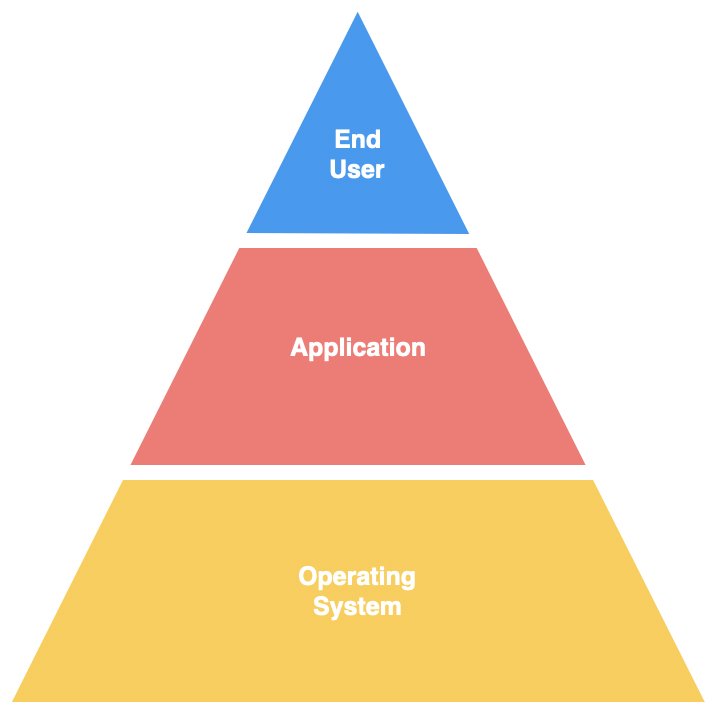
\includegraphics[width=85mm]{model.png} source \footnote{The layers of the android
  security model
  \href{https://proandroiddev.com/the-layers-of-the-android-security-model-90f471015ae6}{Pro
  Android dev}}
\end{center}

Le modèle de sécurité est basé sur le consentement de chacune des
parties. Cela implique que pour qu'une action soit exécutée, les trois
acteurs doivent être d'accord sur cette action.

L'utilisateur attend des deux autres parties d'avoir pris toutes les
mesures nécessaires pour assurer sa sécurité. Il est logique de
minimiser au maximum l'impact de l'utilisateur sur le mécanisme de
sécurité.

En revanche, si l'action nécessite son consentement, c'est \textbf{lui}
qui a le dernier mot. Le système dans son ensemble est alors vulnérable.

\hypertarget{suxe9curity-de-los}{%
\subsection{Sécurity de l'OS}\label{suxe9curity-de-los}}

Le \emph{kernel} est le logiciel central de l'OS. Il gère les ressources
du processeur, la mémoire système, les périphériques système, ainsi que
les systèmes de fichiers et la mise en réseau, et est responsable de la
gestion de tous les processus.

Il sert de lien entre le logiciel et le matériel.

La sécurité du système d'exploitation d'\emph{Android} repose sur les
principales fonctionnalités de sécurité suivantes du noyau Linux :

\begin{itemize}
\tightlist
\item
  Isolation de processus.
\item
  Modèle d'autorisation basé sur l'utilisateur.
\item
  Communication inter-processus (IPC).
\end{itemize}

\hypertarget{sandboxing}{%
\subsubsection{Sandboxing}\label{sandboxing}}

Android utilise le modèle d'autorisations Linux
\emph{user-based-permissions} pour isoler les ressources de
l'application. Ce processus est nommé \emph{sandboxing}.

L'objectif du \emph{sandboxing} est d'empêcher les programmes externes
malveillants d'interagir avec l'application:

\begin{itemize}
\tightlist
\item
  Les composants internes de l'OS sont protégés par le mécanisme de
  sandboxing.
\item
  Les vulnérabilités exposées par une application ne peuvent pas être
  exploitées pour accéder au système externe.
\item
  La communication sécurisée entre les applications est assurée par la
  protection Linux \emph{user-based-permissions}.
\end{itemize}

Contrairement aux systèmes d'exploitation traditionnels, par ex. MacOS
et Windows, Android utilise le concept d'ID utilisateur (UID) pour gérer
le contrôle d'accès d'une application et non le contrôle d'accès de
l'utilisateur du système.

Il est interdit à une application d'accéder aux données ou aux
fonctionnalités du système d'une autre application sans les
autorisations nécessaires.

L'application est en \emph{sandboxing} au niveau du noyau, il est donc
\textbf{garanti} que l'application est isolée du reste du système, quel
que soit l'environnement de développement spécifique, les langages de
programmation ou les API utilisés.

Par défaut, les applications ont un accès limité à l'OS. Cela garantit
qu'une application malveillante ne peut pas accéder au système externe
de l'intérieur.

Pour surmonter les limites du \emph{sandboxing}, l'utilisateur peut
\emph{rooter} l'appareil. Cela implique le contrôle complet de
l'appareil par l'utilisateur. La section suivante détaille ce concept.

\hypertarget{rooting}{%
\subsubsection{Rooting}\label{rooting}}

Sur un système Linux, \textbf{root} est le nom du compte qui a accès à
tous les fichiers et commandes. Étant basé sur Linux, Android a
également ce concept.

Bien que contre-intuitif, \textbf{le propriétaire de l'appareil n'est
pas \emph{root}}. Cette décision de conception a été prise pour des
raisons de sécurité.

Si le propriétaire était capable de faire quoi que ce soit dans le
système, il serait plus facile pour les applications malveillantes de
prendre le contrôle de l'ensemble du système en incitant l'utilisateur à
lui accorder les mêmes autorisations.

Néanmoins, Android est conçu pour être ouvert. Par conséquent,
l'utilisateur est autorisé à rooter le téléphone, c'est-à-dire à passer
à l'utilisateur root.

Il faut savoir qu'après le \emph{rooting}, seules les mesures de
sécurité appliquées par le système d'exploitation sont présentes. Cela
signifie l'ensemble du système est entre les mains de l'utilisateur,
qu'il contrôle tout et qu'il dispose des systèmes de sécurité conçus. 
C'est évidemment une vulnérabilité de plus, mais aussi une liberté supplémentaire.

\hypertarget{android-verified-boot}{%
\subsubsection{Android Verified Boot}\label{android-verified-boot}}

\textbf{Android Verified Boot} s'efforce de s'assurer que tout le code
exécuté provient d'une source fiable (généralement des OEM \footnote{Acronyme:
  original equipment manufacturer} d'appareils), plutôt que d'un
attaquant ou d'une version ``corrompue'' d'OS.

À l'instar de la technologie \emph{Blockchain},, il établit une
\textbf{chaîne de confiance} complète, à partir d'une racine de
confiance protégée par le matériel jusqu'au chargeur de démarrage, à la
partition de démarrage et à d'autres partitions vérifiées, y compris les
partitions système, fournisseur et éventuellement \emph{OEM}.

Lors du démarrage de l'appareil, chaque étape vérifie l'intégrité et
l'authenticité de l'étape suivante avant de continuer l'exécution. Si
l'un des composants de la chaîne est altéré, toute la chaîne est
invalidée et l'utilisateur est averti.

Ce système est fondamental dans tout modèle de sécurité actuel. C'est
sur lui que l'intégrité et l'authenticité du système et de la chaîne de
démarrage sont assurés. La condition est que le bootloader demeure
verrouillé. Il protège de toute forme d'altération par un attaquant
physique ou non:

\begin{itemize}
\tightlist
\item
  Les attaques \emph{evil maid}, autrement dit par possession physique.
\item
  La persistance de \emph{malwares}, de \emph{rootkits}.
\item
  Les attaques par \emph{rollback}, qui consistent à retourner sur des
  versions antérieures du système pour exploiter une faille.
\end{itemize}

\hypertarget{android-verified-boot-flow}{%
\paragraph{Android Verified Boot
Flow}\label{android-verified-boot-flow}}

\begin{flushleft}
L'état de l'appareil peut être l'un des suivants:
\end{flushleft}

\begin{itemize}
\item
  \textbf{LOCKED}: aucun logiciel personnalisé ne peut être flashé sur
  l'appareil et la vérification du démarrage est active.
\item
  \textbf{UNLOCKED}: le logiciel personnalisé peut être flashé sur
  l'appareil et la vérification du démarrage est inactive.
\end{itemize}

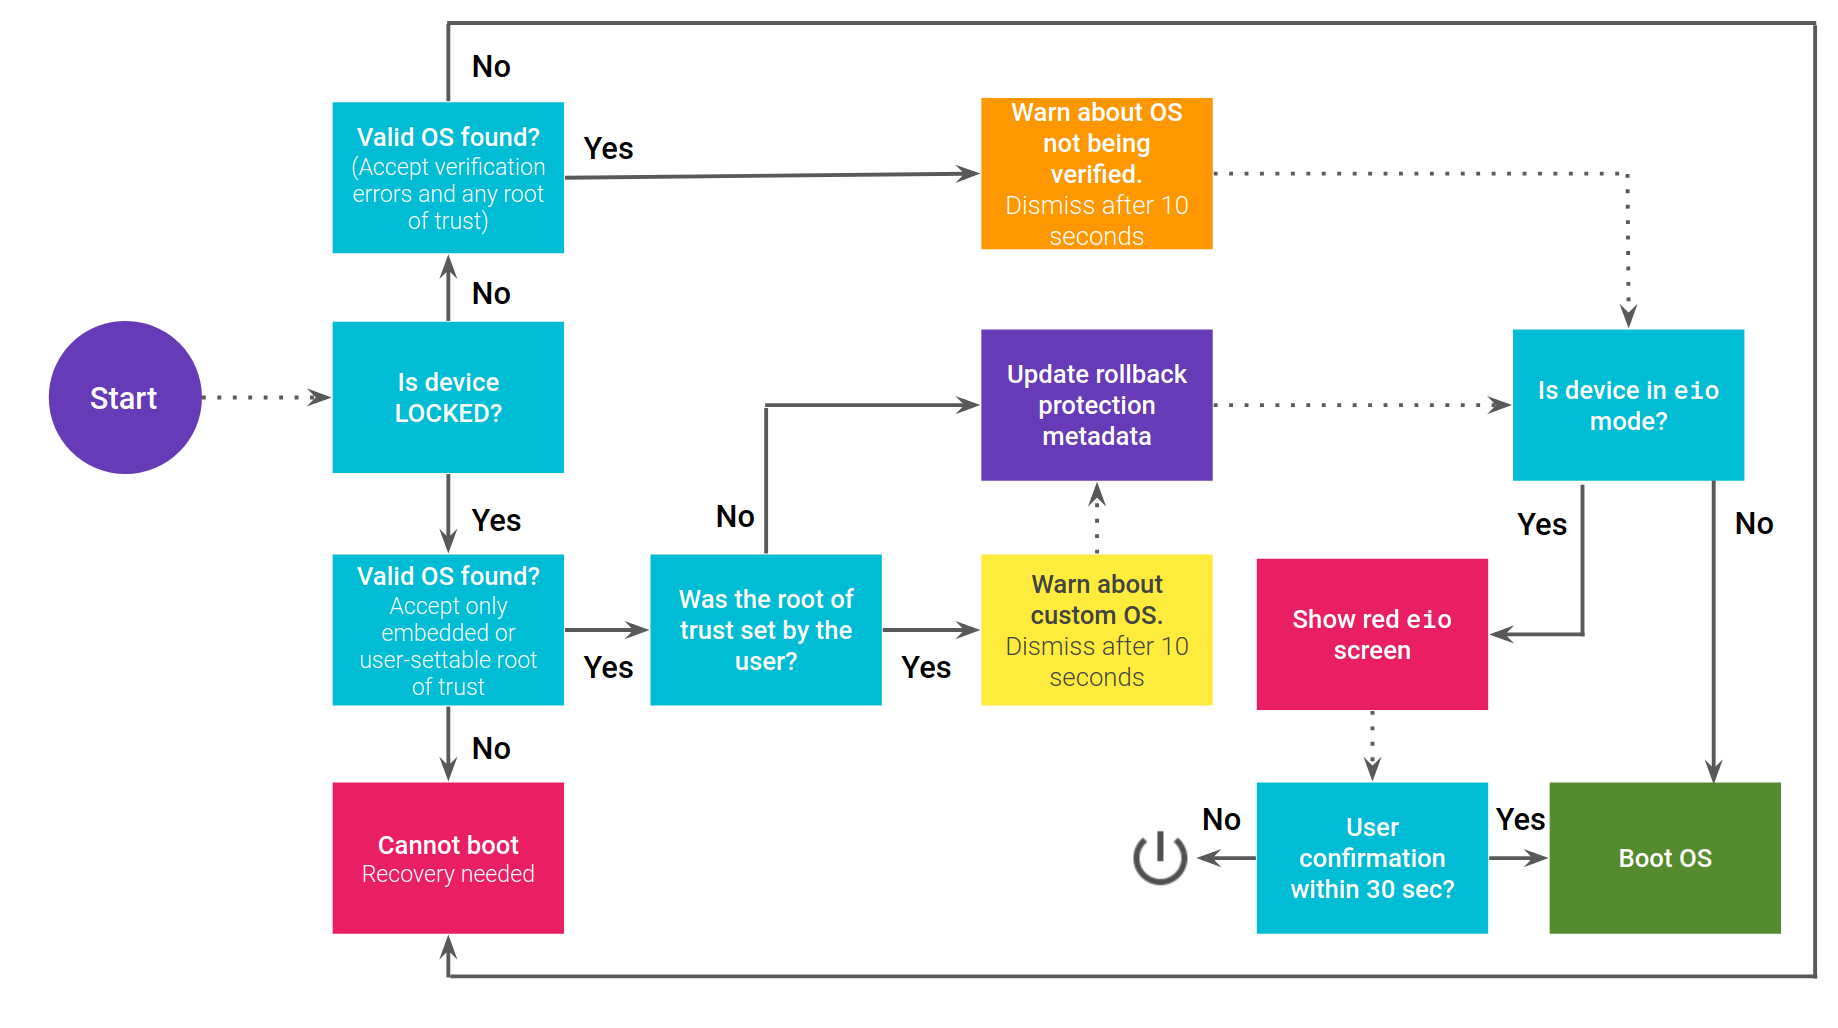
\includegraphics{verified_boot.png} source \footnote{Page 26, Figure 2,
  RENÉ MAYRHOFER, Google and Johannes Kepler University Linz \& co.,
  \href{https://arxiv.org/pdf/1904.05572.pdf}{The Android platform
  Security Model}}

\emph{Root of trust} est une clé cryptographique utilisée pour signer la
copie Android qui s'exécute sur l'appareil. \footnote{Wikipédia,
  \href{https://source.android.com/security/verifiedboot/device-state\#:~:text=Root\%20of\%20trust\%20is\%20the,of\%20Android\%20intended\%20for\%20distribution.}{Root
  of trust}}

Cette clé fait partie du \emph{Verified Boot}. En tant qu'utilisateur,
il est possible de remplacer cette clé afin d'exécuter des versions
personnalisées d'Android.

Ainsi, il est possible de conserver le mécanisme de \emph{Verified Boot}
même si une version différente du système d'exploitation est utilisée.

Android fournit en permanence des mises à jour de sécurité mineures aux
côtés des principales fournies avec chaque nouvelle version d'Android.

Les mises à jour mineures corrigent généralement les vulnérabilités
découvertes.

\hypertarget{faille-possible}{%
\subsubsection{Faille possible}\label{faille-possible}}

Un attaquant pourrait essayer de rétrograder la version d'Android
exécutée sur l'appareil afin d'exploiter les vulnérabilités qui ont été
corrigées. Cette classe d'attaques est atténuée par le système de
\emph{Rollback Protection}. \emph{Rollback Protection} fait aussi partie
du \emph{Verified Boot}.

\hypertarget{suxe9curituxe9-des-applications}{%
\subsection{Sécurité des
applications}\label{suxe9curituxe9-des-applications}}

L'aspect sécurité d'une application est souvent négligé, ce qui amène
une application à devenir un vecteur d'attaque, exploité par des acteurs
malveillants.

Plusieurs mécanismes sont mis en place pour rendre le modèle de sécurité
robuste à ce niveau:

\begin{enumerate}
\def\labelenumi{\arabic{enumi}.}
\tightlist
\item
  Système de permissions.
\item
  Stockage des données.
\item
  Interprocess communication.
\item
  Signature de l'application et mitigations, authentificateurs.
\end{enumerate}

\hypertarget{systuxe8me-de-permissions}{%
\subsubsection{Système de permissions}\label{systuxe8me-de-permissions}}

Les applications Android nécessitent le consentement de l'utilisateur
pour effectuer des actions qui pourraient avoir un impact sur d'autres
applications, le système d'exploitation ou l'utilisateur lui-même.

Les autorisations requises par une application sont déclarées dans le
fichier \texttt{AndroidManifest.xml}. Chaque autorisation est spécifiée
dans sa propre balise uses-permission.

Certaines autorisations sont accordées à l'application par défaut
lorsqu'elles sont spécifiées. Cependant, l'autre catégorie
d'autorisations, appelées autorisations dangereuses, nécessite un
consentement spécial de l'utilisateur.

Selon la version d'Android exécutée sur l'appareil, des autorisations
dangereuses sont requises comme:

\begin{itemize}
\tightlist
\item
  \textbf{Autorisations au moment de l'installation} (pour Android 5.1.1
  et versions antérieures):

  \begin{itemize}
  \tightlist
  \item
    lorsqu'une application est installée, l'utilisateur se voit
    présenter la liste de toutes les autorisations requises par
    l'application.
  \end{itemize}
\item
  \textbf{Autorisations d'exécution} (pour Android 6.0 et supérieur):

  \begin{itemize}
  \tightlist
  \item
    lorsqu'une application demande une autorisation, l'utilisateur est
    invité par une boîte de dialogue. Contrairement aux autorisations
    d'installation, les autorisations d'exécution sont généralement
    demandées lorsque la fonctionnalité respective est nécessaire. Par
    exemple, une autorisation de caméra doit être demandée avant que
    l'utilisateur n'essaie de prendre une capture.
  \end{itemize}
\end{itemize}

\hypertarget{stockage-des-donnuxe9es}{%
\subsubsection{Stockage des données}\label{stockage-des-donnuxe9es}}

Le stockage de données est le domaine le plus sensible de la sécurité
d'\emph{Android}. Dans la majorité des attaques, les données sont le but
ultime d'un attaquant. Il est donc vital d'assurer que chaque option de
stockage de données est correctement sécurisée en fonction de la
sensibilité des données enregistrées.

Trois manière de stockées les données sont proposées:

\begin{enumerate}
\def\labelenumi{\arabic{enumi}.}
\item
  \textbf{Stockage interne:} Les données stockées ici ne sont visibles
  que pour l'application correspondante. Les autres applications n'ont
  pas accès aux fichiers stockés dans le répertoire de l'application
  respective. Lorsque l'application est désinstallée, toutes les données
  stockées sont effacées.
\item
  \textbf{Stockage externe:} Les données stockées dans le stockage
  externe sont globalement lisibles et inscriptibles. Cela signifie que
  n'importe quelle application peut lire ou écrire les fichiers stockés
  ici. Par conséquent, il est nécessaire que les informations sensibles
  de l'application n'y soit pas stockées. Cependant, dans le cas où les
  informations peuvent être sauvegardées publiquement en toute sécurité,
  il est nécessaire d'effectuer les validations nécessaires lors de la
  relecture. Puisque les données peuvent être modifiées par d'autres
  applications ou attaquants, il n'est pas possible de savoir si les
  données écrites précédemment ne se sont pas transformées en un
  logiciel malveillant chargé dynamiquement.
\item
  \textbf{Fournisseurs de contenu:} Ils fournissent une abstraction des
  données stockées. Avec l'utilisation de fournisseurs de contenu, le
  contrôle sur les autorisations de lecture et d'écriture est élargi. Si
  plusieurs applications sont sous la même signature, il est possible de
  partager des données entre elles avec l'utilisation d'un fournisseur
  de contenu, afin que les données ne soient visibles qu'entre ces
  applications.
\end{enumerate}

L'introduction de \emph{Scoped Storage}, dans Android 10, a éliminé la
plupart des risques associés au stockage externe.

\begin{quote}
With Android 10, we adjusted how storage permission works, to give apps
the access they need. This also limits file clutter by encouraging apps
to save files in their designated directories which are cleared when an
app is deleted. \footnote{Scoped Storage,
  \href{https://medium.com/androiddevelopers/modern-user-storage-on-android-e9469e8624f9}{Modern
  user storage on Android}}
\end{quote}

Dans le cas où il est nécessaire de stocker de manière persistante des
paires \emph{key-values}, nous pouvons utiliser l'API
\texttt{SharedPreferences} fournie par Android.

Il est courant chez les développeurs de stocker les informations
d'identification de l'utilisateur dans \texttt{SharedPreferences}.

Cependant, tout ce qui est stocké peut éventuellement se retrouver entre
les mains d'un attaquant.

C'est pourquoi l'ajout d'une couche de sécurité supplémentaire est
nécessaire en cryptant des données stockées. 
À noter que beaucoup d'applications n'applique pas cette mesure.

Pour chiffrer les données, Android fournit la bibliothèque
\texttt{Security} qui comprend, entre autres, deux classes pour le
chiffrement des données:

\begin{itemize}
\tightlist
\item
  \texttt{EncryptedFile}:

  \begin{itemize}
  \tightlist
  \item
    Fournit une implémentation personnalisée sur
    \texttt{FileInputStream} et \texttt{FileOutputStream}, créant
    efficacement des flux de données plus sécurisés:

    \begin{itemize}
    \tightlist
    \item
      les données sont chiffrées et déchiffrées à chaque opération d'E/S
    \end{itemize}
  \end{itemize}
\item
  \texttt{EncryptedSharedPreferences}:

  \begin{itemize}
  \tightlist
  \item
    Fournit une couche sécurisée sur \texttt{SharedPreferences}. Crypte
    automatiquement les clés et les valeurs à l'aide d'une méthode à
    deux schémas (cryptage symétrique).
  \end{itemize}
\end{itemize}

\hypertarget{interprocess-communication}{%
\subsubsection{Interprocess
communication}\label{interprocess-communication}}

Les mécanismes \emph{IPC} permettent d'appliquer des politiques de
sécurité basées sur la relation entre un processus source et un
processus cible. Android fournit les classes suivantes qui facilitent la
communication interprocessus :

\begin{itemize}
\tightlist
\item
  Intent.
\item
  Binder.
\item
  Messenger.
\end{itemize}

Les mécanismes susmentionnés fonctionnent généralement en conjugaison
avec des \texttt{services} et des \texttt{broadcast\ receivers}.

Les \texttt{Intent} sont le mécanisme incontournable pour transmettre
des données lors du développement d'applications avec plusieurs
activités et services. Les \texttt{Intent} peuvent être
\textbf{explicites} ou \textbf{implicites}.

Les \texttt{Intent} \textbf{explicites} sont conçues pour être reçues
par un composant \textbf{explicite}, d'où son nom.

De cette façon, il est possible de certifier que les données envoyées
par l'\emph{application A} ne sont reçues que par l'\emph{application
B}. De plus, des \texttt{Intent} \textbf{explicites} peuvent être
utilisées pour envoyer des données entre les activités à l'intérieur des
applications.

En revanche, les \texttt{Intent} \textbf{implicites} spécifient une
action générale qui doit être effectuée. Selon l'action, l'\texttt{Intent} peut
inclure certaines données nécessaires à l'action. Les \texttt{Intent}
\textbf{implicites} sont généralement utilisées lorsque l'application ne
peut pas effectuer une action et qu'il est nécessaire de déléguer la
tâche à une application tierce.

\hypertarget{exemple}{%
\paragraph{Exemple}\label{exemple}}

\begin{flushleft}
Pour envoyer un message d'une application à une autre, une intention
avec l'action \texttt{ACTION\_SEND} doit être utilisée.
\end{flushleft}

Toute application qui déclare un \texttt{intent-filter} sur l'action
\texttt{ACTION\_SEND} peut \textbf{intercepter} l'\texttt{Intent}
\textbf{implicite}. Lorsque plusieurs applications peuvent répondre à
un\texttt{Intent} \textbf{implicite}, un sélecteur s'affiche. Dans le
cas où une seule application peut y répondre, elle est sélectionnée
implicitement et aucun sélecteur n'est affiché.

Un risque de sécurité est soulevé lorsqu'un\texttt{Intent}
\textbf{implicite} implique de se lier à un service. L'utilisation d'une
\texttt{Intent} \textbf{implicite} peut permettre à un service
malveillant de répondre à la requête, en interceptant efficacement
toutes les communications.

À partir d'Android 5.0, une exception est levée si l'intention transmise
à la méthode \texttt{bindService} est un \texttt{Intent}
\textbf{implicite}.

\texttt{Binder} et \texttt{Messenger} sont utilisés pour implémenter
l'appel de procédure à distance (RPC) IPC dans Android. Ils fournissent
une interface qui facilite la communication sécurisée entre une
application et un service.

\hypertarget{signature-de-lapplication}{%
\subsubsection{Signature de
l'application}\label{signature-de-lapplication}}

La signature de code offre aux développeurs la possibilité d'identifier
l'auteur d'une application et de la mettre à jour de manière
transparente. Par exemple, les applications qui ne sont pas signées par
un développeur ne peuvent pas être téléchargées sur \emph{Google Play}.
\footnote{Wikipédia,
  \href{https://fr.wikipedia.org/wiki/Signature_numérique}{Signature
  numérique}}

Si un package d'application non signé s'est retrouvé sur l'appareil,
l'application ne peut pas être installée car le gestionnaire de packages
vérifie si le package est signé ou non avant d'installer une
application.

La signature d'application est la première étape du mécanisme de
\emph{sandboxing} d'application.

Un UID est attribué en fonction du certificat utilisé pour signer
l'application.

Si plusieurs applications sont signées à l'aide du même certificat,
elles peuvent spécifier la clé \texttt{android:sharedUserId} dans leur
manifeste afin qu'elles partagent le même \textbf{UID}.

Néanmoins, la clé a été \emph{dépréciée} dans l'\textbf{API 29} car elle
pouvait entraîner un comportement non déterministe lors de
\emph{l'attribution de l'UID}. Son utilisation est donc fortement
déconseillée et peut être supprimée dans les futures versions.

Les applications ont la possibilité de créer des autorisations de
sécurité \emph{protégées par la signature}. De cette façon, les
applications signées \textbf{sous le même certificat}, mais \emph{sous
différents UID et bacs à sable applicatifs}, peuvent accéder à des
fonctionnalités restreintes exposées par l'une ou l'autre.

\hypertarget{exemple-de-malware}{%
\subsection{Exemple de malware}\label{exemple-de-malware}}

\hypertarget{hummingbad-2016}{%
\paragraph{HummingBad (2016)}\label{hummingbad-2016}}

\begin{flushleft}
Créé par la société de publicité chinoise Yingmob, \emph{HummingBad}
\footnote{Check Point Software Technologies, ©2016,
  \href{https://blog.checkpoint.com/wp-content/uploads/2016/07/HummingBad-Research-report_FINAL-62916.pdf}{From
  HummingBad to Worse}} a généré des revenus pour la société
susmentionnée en cliquant automatiquement sur des publicités intrusives.
\end{flushleft}
Cinq mois après sa première découverte, en juillet 2016, une société
multinationale de sécurité informatique, appelée \emph{Check Point}, a
publié un rapport contenant des données sur le malware
\emph{HummingBad}.

Non seulement \emph{HummingBad} a affiché des publicités et simulé des
clics dessus, mais il a également installé des \textbf{applications
frauduleuses} sur l'appareil infecté.

\newpage

Le service responsable des réseaux publicitaires utilisés par les
applications s'appelle \textbf{Se}. Un récepteur de diffusion est
enregistré lorsque le logiciel malveillant est installé. Ce récepteur de
diffusion écoute alors les événements suivants :

\begin{itemize}
\item
  \textbf{USER PRESENT} --- se déclenche lorsque l'appareil est
  déverrouillé
\item
  \textbf{BOOT COMPLETED} - se déclenche une fois que l'utilisateur a
  terminé le démarrage
\item
  \textbf{SCREEN ON} --- se déclenche lorsque l'appareil se réveille et
  devient interactif
\end{itemize}

Lorsqu n'importe lequel des événements mentionnés précédemment est reçu
par le récepteur de diffusion, le service \textbf{Se} démarre.

Voici une partie du code concerné pour illustrer le fonctionnement:

\href{https://gist.github.com/deniskrr/7e1bcccde27ba81d17f074729aba5fb4\#file-receiver-java}{\textbf{Receiver.java}}

\begin{lstlisting}[language=Java]
public void onReceive(Context context, Intent intent) {
        Editor editor = UtilsClass.getInstance().getSharedPreferences(context).edit();
        if (Utilstools.ACTIONIAD.equals(intent.getAction())
                || Utilstools.ACTIONZDT.equals(intent.getAction()) ||
                "android.intent.action.USER_PRESENT".equals(intent.getAction()) ||
                "android.intent.action.BOOT_COMPLETED".equals(intent.getAction()) ||
                "android.intent.action.SCREEN_ON".equals(intent.getAction())) {
            if ("android.intent.action.BOOT_COMPLETED".equals(intent.getAction())) {
                MobclickAgent.onEvent(context, "SSP_ReCreate");
            }
            if (!Utilstools.getInstance().isServiceRunning(context)) {
                context.startService(new Intent(context, Se.class));
            }
        }
  //...
}
\end{lstlisting}

Lorsqu'une publicité est affichée, le processus capture l'événement
\emph{KeyDownEvent} et ne l'envoie pas plus loin si le \emph{keycode}
est l'un des suivants :

\begin{itemize}
\item
  KEYCODE HOME (3)
\item
  KEYCODE BACK (4)
\item
  KEYCODE MENU (82)
\end{itemize}

\href{https://gist.github.com/deniskrr/76499ac07a0190a6f515944ae641d13f\#file-keycapture-java}{\textbf{KeyCapture.java}}

\begin{lstlisting}[language=Java]
public boolean onKeyDown(int keyCode, KeyEvent event) {
    if (keyCode == 4 || keyCode == 82 || keyCode == 3) {
        return false;
    }
    return super.onKeyDown(keyCode, event);
}
\end{lstlisting}

Sans pouvoir utiliser les commandes de navigation, l'utilisateur est
\textbf{obligé} de traiter l'annonce.

Cependant, si l'utilisateur essaie de fermer la publicité, l'événement
de clic est intercepté et un événement de clic au milieu de l'écran est
envoyé à la place.

\href{https://gist.github.com/deniskrr/40c99e4a7887a4c4d5856fe1466314a2\#file-simulateclick-java}{\textbf{SimulateClick.java}}

\begin{lstlisting}[language=Java]
public void setSimulateClick(final Activity activity) {
    activity.runOnUiThread(new Runnable() {
        public void run() {
            DisplayMetrics dm = activity.getResources().getDisplayMetrics();
            int x = dm.widthPixels / 2;
            int y = dm.heightPixels / 2;
            long downTime = SystemClock.uptimeMillis();
            MotionEvent downEvent = MotionEvent.obtain(downTime, downTime,
                    0, (float) x, (float) y, 0);
            MotionEvent upEvent = MotionEvent.obtain(downTime, downTime,
                    1, (float) x, (float) y, 0);
            activity.getWindow().getDecorView().dispatchTouchEvent(downEvent);
            activity.getWindow().getDecorView().dispatchTouchEvent(upEvent);
            downEvent.recycle();
            upEvent.recycle();
        }
    });
}
\end{lstlisting}

Dans un premier temps, \emph{HummingBad} va tenter d'accéder à des
droits \textbf{root} du téléphone en utilisant des failles.

S'il n'y parvient pas, il va alors lancer un deuxième processus
d'attaque en émettant une fausse notification de mise à jour système.

En la validant l'utilisateur va alors lui donner des droits et des accès
privilégiés à différents points du téléphone. Pour les deux vecteurs
d'attaque, le résultat est le même, HummingBad va afficher des campagnes
de publicité issues de \emph{Yingmob} et télécharger des fichiers .apk.
Le malware va même jusqu'à modifier le numéro IMEI du téléphone pour
améliorer le nombre d'affichage de publicité et d'installation
d'applications.

\newpage

\hypertarget{conclusion}{%
\section{Conclusion}\label{conclusion}}

Tout comme les ordinateurs, les smartphones sont des cibles privilégiées d'attaques. De plus en plus d'utilisateurs et d'entreprises utilisent régulièrement des smartphones comme outils de communication. Mais ils les utilisent aussi pour la planification, la gestion et l'organisation de leurs vies professionnelle et privée, ce qui est autrement plus confidentiel. C'est donc toujours et même de plus en plus un sujet actuel sur lequel les entreprises et les particuliers ont besoin de personnes pouvant répondre a leurs besoins de sécurité. 

En effet, les smartphones collectent et compilent un nombre croissant d'informations sensibles dont l'accès doit être contrôlé afin de protéger la vie privée de l'usager ainsi que ce qui est du domaine de la propriété intellectuelle de l'entreprise. Android étant un système ouvert, c'est le candidat de choix pour être accueilli par l'écrasante majorité des smartphones qui fonctionnent actuellement. Malheureusement, cette forme de qualité est aussi sa faiblesse.

Les constructeurs (OEMs) modifient assez intensivement Android en y intégrant des services tiers, qui ne font que contribuer à agrandir la surface d'attaque et introduire des \emph{bugs}. Ces OEMs vont même jusqu'à réduire la sécurité globale : Asus par exemple rend la politique SELinux plus permissive, ce qui va à contre sens du modèle de sécurité de base, et beaucoup de smartphones n'implémentent pas \emph{android verified boot} correctement.  Malgré un modèle profondément pensé pour la sécurité, les constructeurs tiers l'affaiblissent considérablement. Le modèle de sécurité d'Android actuel souffre aussi de la fragmentation. En rendant le système modulaire, il persiste à travers les mises à jour. \footnote{La distribution, sa grande faiblesse,
  \href{https://wonderfall.space/modele-securite-mobile/}{la fragmentation}}

En ce qui concerne le hardware, les modèles de smartphones Pixels obtiennent la meilleure note. Il y a peu de modifications à AOSP et toutes les sécurités sont bien implémentées. Aussi, le hardware est pensé pour tirer profit des dernières API disponibles sur Android (exemple avec StrongBox). Ils ont également un suivi convenable dans le temps et avec transparence : 3 ans en moyenne de mises à jour majeures avec patchs de sécurité livrés chaque début de mois, avec rapidité. De plus, ils intègrent un kernel Linux compilé par clang avec le Control Flow Integrity, ce qui n'est pas le cas de la majorité des modèles.

Modifier le système de base pour installer des éléments par du rooting est à éviter. Android se fonde sur le principe du moindre privilège et n'emploie pas lui-même des privilèges non-restreints. Aussi, les ROMs customs sont négligentes du modèle de sécurité; bootloader déverrouillé (car elles ne sont pas reconnues comme OS valide), patchs de sécurités partiellement implémentés pour le matériel, entre autres failles.

\newpage

\hypertarget{bibliographie}{%
\section{Bibliographie}\label{bibliographie}}

{[}1{]} Bruno Camus, Rapports de stages et mémoires, Les éditions
d'organisation, 1989. (Bibliothèque ENSPS : 808.06 CAM)

{[}2{]} Règles typographiques en usage à l'Imprimerie nationale,
Imprimerie nationale, troisième édition, 1994.

{[}3{]}
\href{https://github.com/Wandmalfarbe/pandoc-latex-template}{Eisvogel},
Latex template, Copyright (c) 2017 - 2021, Pascal Wagler, 2014 - 2021,
John MacFarlane, open source licensed under the BSD 3-Clause License.

{[}4{]} Check Point Software Technologies, ©2016,
\href{https://blog.checkpoint.com/wp-content/uploads/2016/07/HummingBad-Research-report_FINAL-62916.pdf}{From
HummingBad to Worse}

{[}5{]} Wikipédia, Security-Enhanced Linux,
\href{https://fr.wikipedia.org/wiki/SELinux}{\textbf{SELinux}}

{[}6{]} Wonderfall,
\href{https://wonderfall.space/modele-securite-mobile/}{Modèle sécurité
mobile}

{[}7{]} Android,
\href{https://source.android.com/security/verifiedboot}{Verified Boot}

{[}8{]} Android, Scoped Storage,
\href{https://medium.com/androiddevelopers/modern-user-storage-on-android-e9469e8624f9}{Modern
user storage on Android}

{[}9{]} Wikipédia,
\href{https://fr.wikipedia.org/wiki/Signature_numérique}{Signature
numérique}

{[}10{]} Android Central. Root Your Android Phone: What is Root \& How
To. \href{https://www.androidcentral.com/root}{Root}

\end{document}
